\documentclass{zkdl-presentation-template}

\usepackage[T1]{fontenc}
\usepackage{kerkis}
\usepackage{kmath}
%\usepackage{concmath}
\usepackage{centernot}

\newcommand\leftarrowS{\leftarrow\joinrel\smalldollar}
\newcommand\rightarrowS{\smalldollar\joinrel\rightarrow}

\makeatletter
\newcommand{\smalldollar}{\mathrel{\mathpalette\small@dollar\relax}}
\newcommand{\small@dollar}[2]{%
  \vcenter{\hbox{%
    $#1\textnormal{\fontsize{0.7\dimexpr\f@size pt}{0}\selectfont\$}$%
  }}%
}
\makeatother

\tikzset{
    grid_cell/.style={
        rectangle, 
        draw=black, 
        very thick,
        minimum size=0.75cm, 
        font=\large\bfseries
    },
    grid_label/.style={
        font=\small
    },
    hypercube_highlight/.style={
        fill=gray!40
    }
}

% Define values for x_1 to x_8
\newcommand{\xval}[1]{%
\ifcase#1
    % case 0 (won't be used)
    \or 1  % 1st
    \or 2  % 2nd
    \or 0  % 3rd
    \or 1  % 4th
    \or 0  % 5th
    \or 2  % 6th
    \or 0  % 7th
    \or 1  % 8th
\fi
}

\title[GKR \& Memory Checking]{\textbf{GKR Protocol. Offline Memory Checking}}
\author{Distributed Lab}
\date{July 17, 2025}
\homepage{zkdl-camp.github.io}
\github{ZKDL-Camp}

\begin{document}
    \frame {
        \tikz [remember picture,overlay]
        \node at
            ([yshift=1.5cm,xshift=-1.5cm]current page.south east) 
            %or: (current page.center)
            {
\includegraphics[width=60pt]{images/logo.png}};
        \titlepage
    }

	\section{Introduction}

    \begin{frame}{Recap: Multivariate World and Sum-Check}
        \begin{figure}
            \centering
            
\includegraphics[width=0.55\textwidth]{images/lecture_15/bad_boy.jpg}
        \end{figure}
        \begin{columns}
            \begin{column}{0.5\textwidth}
                \textcolor{blue!70!black}{\begin{center}
                    \textbf{Univariate World:}
                \end{center}
                \[p(X) = q(X)\prod_{u \in \Omega}(X-u)\]}
            \end{column}
            \begin{column}{0.5\textwidth}
                \textcolor{green!50!black}{
                \begin{center}
                    \textbf{Multivariate World:}
                \end{center}
                \[\sum_{\mathbf{b} \in \{0,1\}^{\ell}} f(b_1,\dots,b_{\ell}) = H\]}
            \end{column}
        \end{columns}

        \vspace{-10px}
        
        \textbf{Goal:} build the set of constraints that boil down to \textbf{Sum-Check}:
        \begin{equation*}
            \textcolor{green!50!black}{\sum_{(b_1,\dots,b_{\ell}) \in \{0,1\}^{\ell}} f(b_1,\dots,b_{\ell}) = H}
        \end{equation*}

        \textbf{Cost:} Quasilinear prover, logarithmic verifier and proof size.
    \end{frame}

    \section{GKR Protocol}

    \begin{frame}{Motivation}
        \textcolor{blue!70!black}{\textbf{Goal:} Build sumcheck-based version of the circuit
        arithmetization.}

        Suppose we are given the \textbf{layered} fan-in two arithmetical
        circuit $\mathtt{C}: \mathbb{F}^n \to \mathbb{F}^m$ of size $S$ (number
        of gates). The \textit{layered} here means that the circuit $\mathtt{C}$
        can be decomposed into $d$ layers (note that GKR can be generalized to
        the unstructured arithmetical circuits as well). 
        \begin{figure}
            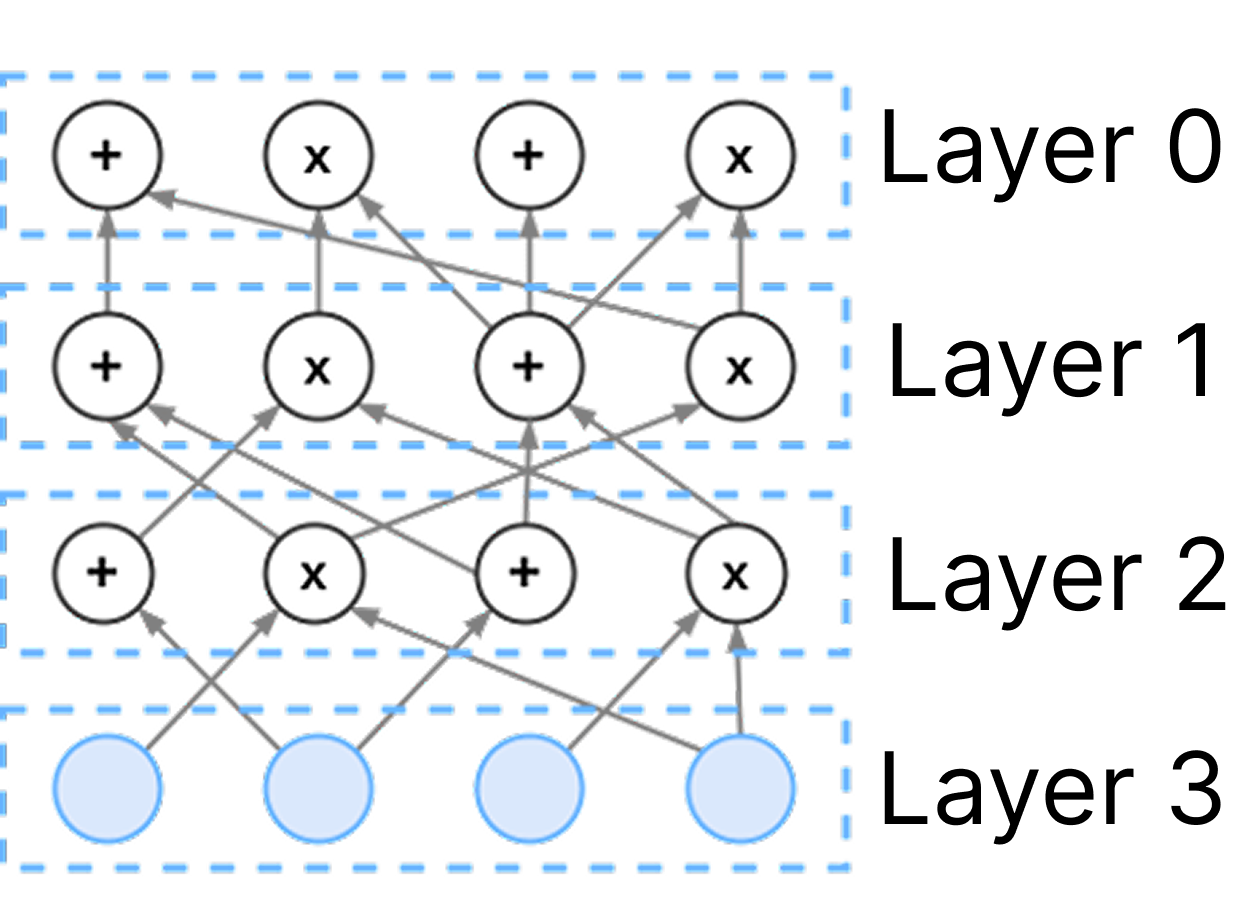
\includegraphics[width=0.5\linewidth]{images/lecture_16/structured.png}
            \caption{Layered Circuit Structure of $d=4$ layers.}
        \end{figure}
    \end{frame}

    \begin{frame}{Spoilers on Performance}        
        The GKR protocol allows 
        to achieve the following performance:
        \begin{itemize}
            \item The communication consists of $\mathcal{O}(d \cdot \mathsf{polylog}(S))$ field elements.
            \item The verifier runs in $\mathcal{O}(n + d \cdot \mathsf{polylog}(S))$ time.
            \item The prover runs in $\mathcal{O}(\mathsf{poly}(S))$ time.
            \item The soundness error is just $\mathcal{O}(d \log(S) / |\mathbb{F}|)$.
        \end{itemize}

        \textbf{Assumptions:}
        \begin{itemize}
            \item Assume we have $d$ rounds in total. Output layer is the
            $0^{\text{th}}$ layer.
            \item Each layer consists of $S_i$ gates.
            \item Assume $S_i=2^{v_i}$ is the power of two
        \end{itemize}
    \end{frame}

    \begin{frame}{Concrete Circuit}
        \begin{figure}[H]
        \centering
        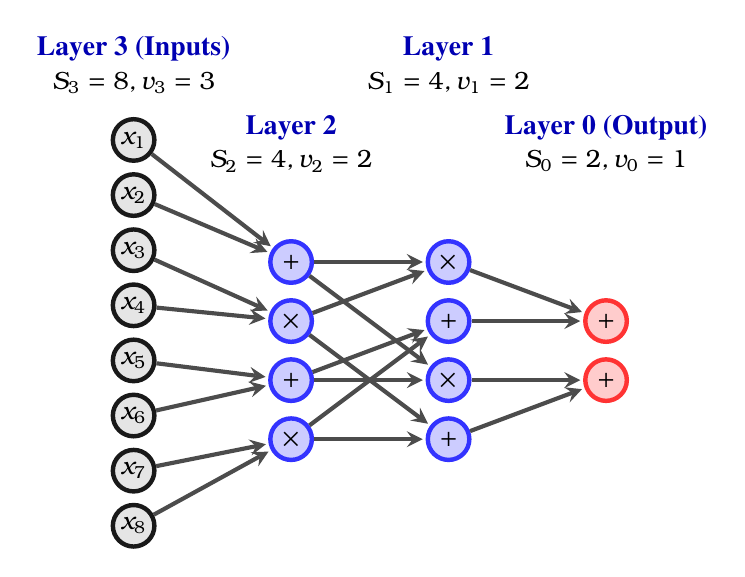
\begin{tikzpicture}[
            % Define styles for different parts of the circuit
            input/.style={circle, ultra thick, draw=gray!20!black, fill=gray!20, minimum size=15pt, inner sep=0pt},
            gate/.style={circle, ultra thick, draw=blue!80, fill=blue!20, minimum size=15pt, inner sep=0pt},
            output/.style={circle, ultra thick, draw=red!80, fill=red!20, minimum size=15pt, inner sep=0pt},
            conn/.style={-stealth, draw=black!70, shorten >=1pt, line width=1.5pt}
        ]

        % --- Layer Labels ---
        \node[font=\bfseries, align=center] at (0, 7.75) {\textcolor{blue!70!black}{Layer 3 (Inputs)} \\ $S_3=8,v_3=3$};
        \node[font=\bfseries, align=center] at (2, 6.75) {\textcolor{blue!70!black}{Layer 2}\\ $S_2=4,v_2=2$};
        \node[font=\bfseries, align=center] at (4, 7.75) {\textcolor{blue!70!black}{Layer 1} \\ $S_1=4,v_1=2$};
        \node[font=\bfseries, align=center] at (6, 6.75) {\textcolor{blue!70!black}{Layer 0 (Output)} \\ $S_0=2, v_0=1$};


        % --- Layer 0: Input Nodes (8) ---
        % We use a \foreach loop to create the 8 input nodes vertically
        \foreach \i in {1,...,8} {
            \node[input] (l0-\i) at (0, 7.5 - 0.7*\i) {$x_{\i}$};
        }

        % --- Layer 1: Gate Nodes (4) ---
        % Alternating between + and x gates
        \node[gate] (l1-1) at (2, 5.25) {$+$};
        \node[gate] (l1-2) at (2, 4.5) {$\times$};
        \node[gate] (l1-3) at (2, 3.75) {$+$};
        \node[gate] (l1-4) at (2, 3.0) {$\times$};

        % --- Layer 2: Gate Nodes (4) ---
        \node[gate] (l2-1) at (4, 5.25) {$\times$};
        \node[gate] (l2-2) at (4, 4.5) {$+$};
        \node[gate] (l2-3) at (4, 3.75) {$\times$};
        \node[gate] (l2-4) at (4, 3.0) {$+$};

        % --- Layer 3: Output Nodes (2) ---
        \node[output] (l3-1) at (6, 4.5) {$+$};
        \node[output] (l3-2) at (6, 3.75) {$+$};


        % --- Connections ---

        % Connections from Layer 0 to Layer 1
        \foreach \i in {1,...,4} {
            \pgfmathtruncatemacro{\j}{2 * \i - 1} % Calculate first source node index
            \pgfmathtruncatemacro{\k}{2 * \i}     % Calculate second source node index
            \draw[conn] (l0-\j) -- (l1-\i);
            \draw[conn] (l0-\k) -- (l1-\i);
        }

        % Connections from Layer 1 to Layer 2
        % This wiring pattern creates a mixing of the signals
        \draw[conn] (l1-1) -- (l2-1);
        \draw[conn] (l1-2) -- (l2-1);

        \draw[conn] (l1-3) -- (l2-2);
        \draw[conn] (l1-4) -- (l2-2);

        \draw[conn] (l1-1) -- (l2-3);
        \draw[conn] (l1-3) -- (l2-3);

        \draw[conn] (l1-2) -- (l2-4);
        \draw[conn] (l1-4) -- (l2-4);

        % Connections from Layer 2 to Layer 3
        \draw[conn] (l2-1) -- (l3-1);
        \draw[conn] (l2-2) -- (l3-1);

        \draw[conn] (l2-3) -- (l3-2);
        \draw[conn] (l2-4) -- (l3-2);

        \end{tikzpicture}
        \caption{Example layered arithmetical circuit $\mathtt{C}: \mathbb{F}^8 \to
        \mathbb{F}^2$ with $d=3$ layers.}
        \end{figure}
    \end{frame}

    \begin{frame}{Gates Encoding}
        \textcolor{blue!70!black}{\textbf{Gates Encoding.}} Suppose $W_i: \{0,1\}^{v_i} \to \mathbb{F}$ is
        structured so that it outputs the value of the $i$-th layer gate given the gate
        label. Assume MLE of $W_i$ is
        $\widetilde{W}_i: \mathbb{F}^{v_i} \to \mathbb{F}$.

        \begin{center}
        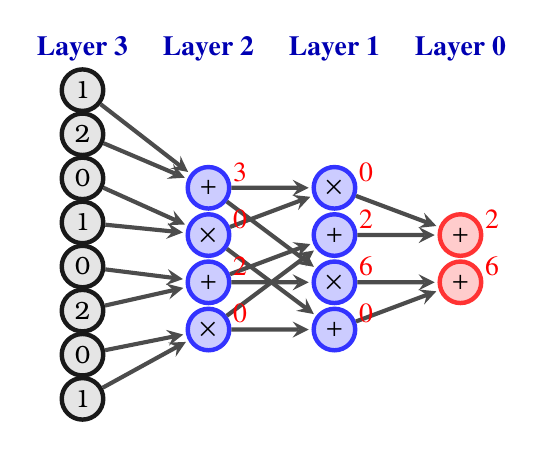
\begin{tikzpicture}[
            % Define styles for different parts of the circuit
            input/.style={circle, ultra thick, draw=gray!20!black, fill=gray!20, minimum size=15pt, inner sep=0pt},
            gate/.style={circle, ultra thick, draw=blue!80, fill=blue!20, minimum size=15pt, inner sep=0pt},
            output/.style={circle, ultra thick, draw=red!80, fill=red!20, minimum size=15pt, inner sep=0pt},
            conn/.style={-stealth, draw=black!70, shorten >=1pt, line width=1.5pt},
            scale=0.8
        ]

        % --- Layer Labels ---
        \node[font=\bfseries, align=center] at (0, 7.45) {\textcolor{blue!70!black}{Layer 3}};
        \node[font=\bfseries, align=center] at (2, 7.45) {\textcolor{blue!70!black}{Layer 2}};
        \node[font=\bfseries, align=center] at (4, 7.45) {\textcolor{blue!70!black}{Layer 1}};
        \node[font=\bfseries, align=center] at (6, 7.45) {\textcolor{blue!70!black}{Layer 0}};

        % --- Layer 0: Input Nodes (8) ---
        % We use a \foreach loop to create the 8 input nodes vertically
        \foreach \i in {1,...,8} {
            \node[input] (l0-\i) at (0, 7.5 - 0.7*\i) {$\xval{\i}$};
        }

        % --- Layer 1: Gate Nodes (4) ---
        % Alternating between + and x gates
        \node[gate] (l1-1) at (2, 5.25) {$+$};

        \node[gate] (l1-2) at (2, 4.5) {$\times$};
 
        \node[gate] (l1-3) at (2, 3.75) {$+$};

        \node[gate] (l1-4) at (2, 3.0) {$\times$};

        % --- Layer 2: Gate Nodes (4) ---
        \node[gate] (l2-1) at (4, 5.25) {$\times$};
        \node[gate] (l2-2) at (4, 4.5) {$+$};
        \node[gate] (l2-3) at (4, 3.75) {$\times$};
        \node[gate] (l2-4) at (4, 3.0) {$+$};

        % --- Layer 3: Output Nodes (2) ---
        \node[output] (l3-1) at (6, 4.5) {$+$};
        \node[output] (l3-2) at (6, 3.75) {$+$};


        % --- Connections ---

        % Connections from Layer 0 to Layer 1
        \foreach \i in {1,...,4} {
            \pgfmathtruncatemacro{\j}{2 * \i - 1} % Calculate first source node index
            \pgfmathtruncatemacro{\k}{2 * \i}     % Calculate second source node index
            \draw[conn] (l0-\j) -- (l1-\i);
            \draw[conn] (l0-\k) -- (l1-\i);
        }

        % Connections from Layer 1 to Layer 2
        % This wiring pattern creates a mixing of the signals
        \draw[conn] (l1-1) -- (l2-1);
        \draw[conn] (l1-2) -- (l2-1);

        \draw[conn] (l1-3) -- (l2-2);
        \draw[conn] (l1-4) -- (l2-2);

        \draw[conn] (l1-1) -- (l2-3);
        \draw[conn] (l1-3) -- (l2-3);

        \draw[conn] (l1-2) -- (l2-4);
        \draw[conn] (l1-4) -- (l2-4);

        % Connections from Layer 2 to Layer 3
        \draw[conn] (l2-1) -- (l3-1);
        \draw[conn] (l2-2) -- (l3-1);

        \draw[conn] (l2-3) -- (l3-2);
        \draw[conn] (l2-4) -- (l3-2);

        % Values in gates, layer 2
        \node at (2.5, 5.5) {\textcolor{red}{3}};
        \node at (2.5, 4.75) {\textcolor{red}{0}};
        \node at (2.5, 4.0) {\textcolor{red}{2}};
        \node at (2.5, 3.25) {\textcolor{red}{0}};

        % Values in gates, layer 1
        \node at (4.5, 5.5) {\textcolor{red}{0}};
        \node at (4.5, 4.75) {\textcolor{red}{2}};
        \node at (4.5, 4.0) {\textcolor{red}{6}};
        \node at (4.5, 3.25) {\textcolor{red}{0}};

        % Values in gates, layer 0
        \node at (6.5, 4.75) {\textcolor{red}{2}};
        \node at (6.5, 4.0) {\textcolor{red}{6}};
        \end{tikzpicture}
        \end{center}
        \vspace{-12.5px}
        \begin{gather*}
            W_1(0, 0) = 0, \quad W_1(0, 1) = 2, \quad W_1(1, 0) = 6, \quad W_1(1, 1) = 0 \\
            \textbf{MLE Extension:} \quad \widetilde{W}_1(X_1,X_2) = 2(1-X_1)X_2 + 6X_1(1-X_2)
        \end{gather*}
    \end{frame}

    \begin{frame}{Wiring Encoding}
        \textcolor{green!80!black}{\textbf{Wiring Predicates.}} $\mathsf{in}_{1,i}, \mathsf{in}_{2,i}:
        \{0,1\}^{v_i} \to \{0,1\}^{v_{i+1}}$ indicate which pairs of
        wiring are connected to the $i^{\text{th}}$ layer gate from the layer $i+1$.

        \begin{center}
        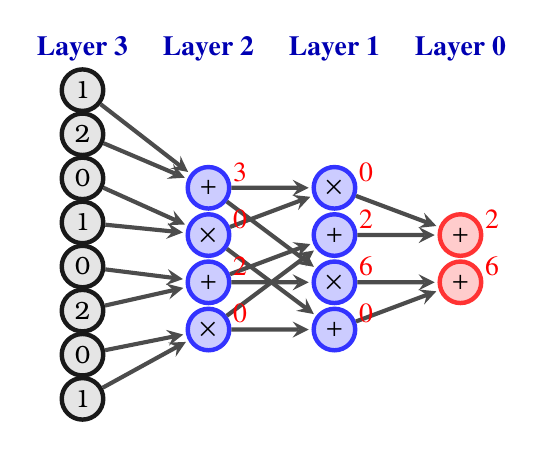
\begin{tikzpicture}[
            % Define styles for different parts of the circuit
            input/.style={circle, ultra thick, draw=gray!20!black, fill=gray!20, minimum size=15pt, inner sep=0pt},
            gate/.style={circle, ultra thick, draw=blue!80, fill=blue!20, minimum size=15pt, inner sep=0pt},
            output/.style={circle, ultra thick, draw=red!80, fill=red!20, minimum size=15pt, inner sep=0pt},
            conn/.style={-stealth, draw=black!70, shorten >=1pt, line width=1.5pt},
            scale=0.8
        ]

        % --- Layer Labels ---
        \node[font=\bfseries, align=center] at (0, 7.45) {\textcolor{blue!70!black}{Layer 3}};
        \node[font=\bfseries, align=center] at (2, 7.45) {\textcolor{blue!70!black}{Layer 2}};
        \node[font=\bfseries, align=center] at (4, 7.45) {\textcolor{blue!70!black}{Layer 1}};
        \node[font=\bfseries, align=center] at (6, 7.45) {\textcolor{blue!70!black}{Layer 0}};

        % --- Layer 0: Input Nodes (8) ---
        % We use a \foreach loop to create the 8 input nodes vertically
        \foreach \i in {1,...,8} {
            \node[input] (l0-\i) at (0, 7.5 - 0.7*\i) {$\xval{\i}$};
        }

        % --- Layer 1: Gate Nodes (4) ---
        % Alternating between + and x gates
        \node[gate] (l1-1) at (2, 5.25) {$+$};

        \node[gate] (l1-2) at (2, 4.5) {$\times$};
 
        \node[gate] (l1-3) at (2, 3.75) {$+$};

        \node[gate] (l1-4) at (2, 3.0) {$\times$};

        % --- Layer 2: Gate Nodes (4) ---
        \node[gate] (l2-1) at (4, 5.25) {$\times$};
        \node[gate] (l2-2) at (4, 4.5) {$+$};
        \node[gate] (l2-3) at (4, 3.75) {$\times$};
        \node[gate] (l2-4) at (4, 3.0) {$+$};

        % --- Layer 3: Output Nodes (2) ---
        \node[output] (l3-1) at (6, 4.5) {$+$};
        \node[output] (l3-2) at (6, 3.75) {$+$};


        % --- Connections ---

        % Connections from Layer 0 to Layer 1
        \foreach \i in {1,...,4} {
            \pgfmathtruncatemacro{\j}{2 * \i - 1} % Calculate first source node index
            \pgfmathtruncatemacro{\k}{2 * \i}     % Calculate second source node index
            \draw[conn] (l0-\j) -- (l1-\i);
            \draw[conn] (l0-\k) -- (l1-\i);
        }

        % Connections from Layer 1 to Layer 2
        % This wiring pattern creates a mixing of the signals
        \draw[conn] (l1-1) -- (l2-1);
        \draw[conn] (l1-2) -- (l2-1);

        \draw[conn] (l1-3) -- (l2-2);
        \draw[conn] (l1-4) -- (l2-2);

        \draw[conn] (l1-1) -- (l2-3);
        \draw[conn] (l1-3) -- (l2-3);

        \draw[conn] (l1-2) -- (l2-4);
        \draw[conn] (l1-4) -- (l2-4);

        % Connections from Layer 2 to Layer 3
        \draw[conn] (l2-1) -- (l3-1);
        \draw[conn] (l2-2) -- (l3-1);

        \draw[conn] (l2-3) -- (l3-2);
        \draw[conn] (l2-4) -- (l3-2);

        % Values in gates, layer 2
        \node at (2.5, 5.5) {\textcolor{red}{3}};
        \node at (2.5, 4.75) {\textcolor{red}{0}};
        \node at (2.5, 4.0) {\textcolor{red}{2}};
        \node at (2.5, 3.25) {\textcolor{red}{0}};

        % Values in gates, layer 1
        \node at (4.5, 5.5) {\textcolor{red}{0}};
        \node at (4.5, 4.75) {\textcolor{red}{2}};
        \node at (4.5, 4.0) {\textcolor{red}{6}};
        \node at (4.5, 3.25) {\textcolor{red}{0}};

        % Values in gates, layer 0
        \node at (6.5, 4.75) {\textcolor{red}{2}};
        \node at (6.5, 4.0) {\textcolor{red}{6}};
        \end{tikzpicture}
        \end{center}
    \end{frame}

    \begin{frame}{Wiring Encoding}
        \textcolor{green!80!black}{\textbf{Wiring Predicates.}} $\mathsf{in}_{1,i}, \mathsf{in}_{2,i}:
        \{0,1\}^{v_i} \to \{0,1\}^{v_{i+1}}$ indicate which pairs of
        wiring are connected to the $i^{\text{th}}$ layer gate from the layer $i+1$.

        \begin{center}
        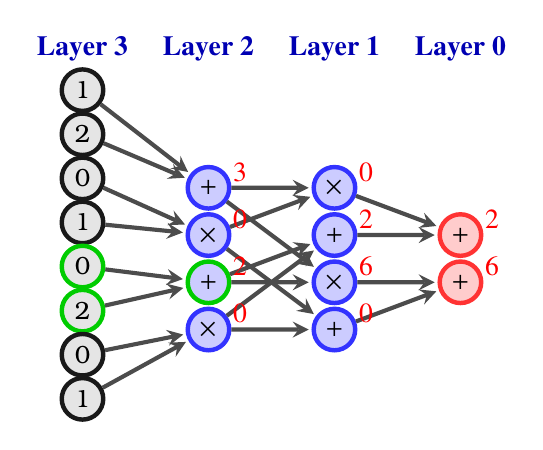
\begin{tikzpicture}[
            % Define styles for different parts of the circuit
            input/.style={circle, ultra thick, draw=gray!20!black, fill=gray!20, minimum size=15pt, inner sep=0pt},
            gate/.style={circle, ultra thick, draw=blue!80, fill=blue!20, minimum size=15pt, inner sep=0pt},
            output/.style={circle, ultra thick, draw=red!80, fill=red!20, minimum size=15pt, inner sep=0pt},
            conn/.style={-stealth, draw=black!70, shorten >=1pt, line width=1.5pt},
            scale=0.8
        ]

        % --- Layer Labels ---
        \node[font=\bfseries, align=center] at (0, 7.45) {\textcolor{blue!70!black}{Layer 3}};
        \node[font=\bfseries, align=center] at (2, 7.45) {\textcolor{blue!70!black}{Layer 2}};
        \node[font=\bfseries, align=center] at (4, 7.45) {\textcolor{blue!70!black}{Layer 1}};
        \node[font=\bfseries, align=center] at (6, 7.45) {\textcolor{blue!70!black}{Layer 0}};

        % --- Layer 0: Input Nodes (8) ---
        % We use a \foreach loop to create the 8 input nodes vertically
        \node[input] (l0-1) at (0, 7.5 - 0.7*1) {$\xval{1}$};
        \node[input] (l0-2) at (0, 7.5 - 0.7*2) {$\xval{2}$};
        \node[input] (l0-3) at (0, 7.5 - 0.7*3) {$\xval{3}$};
        \node[input] (l0-4) at (0, 7.5 - 0.7*4) {$\xval{4}$};
        \node[input, draw=green!80!black] (l0-5) at (0, 7.5 - 0.7*5) {$\xval{5}$};
        \node[input, draw=green!80!black] (l0-6) at (0, 7.5 - 0.7*6) {$\xval{6}$};
        \node[input] (l0-7) at (0, 7.5 - 0.7*7) {$\xval{7}$};
        \node[input] (l0-8) at (0, 7.5 - 0.7*8) {$\xval{8}$};
        % \foreach \i in {1,...,8} {
        %     \node[input] (l0-\i) at (0, 7.5 - 0.7*\i) {$\xval{\i}$};
        % }

        % --- Layer 1: Gate Nodes (4) ---
        % Alternating between + and x gates
        \node[gate] (l1-1) at (2, 5.25) {$+$};

        \node[gate] (l1-2) at (2, 4.5) {$\times$};
 
        \node[gate, draw=green!80!black] (l1-3) at (2, 3.75) {$+$};

        \node[gate] (l1-4) at (2, 3.0) {$\times$};

        % --- Layer 2: Gate Nodes (4) ---
        \node[gate] (l2-1) at (4, 5.25) {$\times$};
        \node[gate] (l2-2) at (4, 4.5) {$+$};
        \node[gate] (l2-3) at (4, 3.75) {$\times$};
        \node[gate] (l2-4) at (4, 3.0) {$+$};

        % --- Layer 3: Output Nodes (2) ---
        \node[output] (l3-1) at (6, 4.5) {$+$};
        \node[output] (l3-2) at (6, 3.75) {$+$};


        % --- Connections ---

        % Connections from Layer 0 to Layer 1
        \foreach \i in {1,...,4} {
            \pgfmathtruncatemacro{\j}{2 * \i - 1} % Calculate first source node index
            \pgfmathtruncatemacro{\k}{2 * \i}     % Calculate second source node index
            \draw[conn] (l0-\j) -- (l1-\i);
            \draw[conn] (l0-\k) -- (l1-\i);
        }

        % Connections from Layer 1 to Layer 2
        % This wiring pattern creates a mixing of the signals
        \draw[conn] (l1-1) -- (l2-1);
        \draw[conn] (l1-2) -- (l2-1);

        \draw[conn] (l1-3) -- (l2-2);
        \draw[conn] (l1-4) -- (l2-2);

        \draw[conn] (l1-1) -- (l2-3);
        \draw[conn] (l1-3) -- (l2-3);

        \draw[conn] (l1-2) -- (l2-4);
        \draw[conn] (l1-4) -- (l2-4);

        % Connections from Layer 2 to Layer 3
        \draw[conn] (l2-1) -- (l3-1);
        \draw[conn] (l2-2) -- (l3-1);

        \draw[conn] (l2-3) -- (l3-2);
        \draw[conn] (l2-4) -- (l3-2);

        % Values in gates, layer 2
        \node at (2.5, 5.5) {\textcolor{red}{3}};
        \node at (2.5, 4.75) {\textcolor{red}{0}};
        \node at (2.5, 4.0) {\textcolor{red}{2}};
        \node at (2.5, 3.25) {\textcolor{red}{0}};

        % Values in gates, layer 1
        \node at (4.5, 5.5) {\textcolor{red}{0}};
        \node at (4.5, 4.75) {\textcolor{red}{2}};
        \node at (4.5, 4.0) {\textcolor{red}{6}};
        \node at (4.5, 3.25) {\textcolor{red}{0}};

        % Values in gates, layer 0
        \node at (6.5, 4.75) {\textcolor{red}{2}};
        \node at (6.5, 4.0) {\textcolor{red}{6}};
        \end{tikzpicture}
        \end{center}
        \vspace{-12.5px}
        \begin{gather*}
            \mathsf{in}_{1,2}(\textcolor{green!80!black}{1,0}) = \textcolor{green!80!black}{(1,0,1)}, \quad \mathsf{in}_{2,2}(\textcolor{green!80!black}{1,0}) = \textcolor{green!80!black}{(1,1,0)}.
        \end{gather*}
    \end{frame}

    \begin{frame}{Operations Encoding}
        \textcolor{magenta}{\textbf{Operations Encodings.}} $\mathsf{add},\mathsf{mul}:
        \{0,1\}^{v_i+2v_{i+1}} \to \{0,1\}$: 
        \vspace{-10px}
        \begin{equation*}
            \mathsf{add}(a,b,c) = 1 \iff (b,c)=(\mathsf{in}_{1,i}(a),
        \mathsf{in}_{2,i}(a)) \; \text{and $a$ is addition gate}
        \end{equation*}

        \begin{center}
        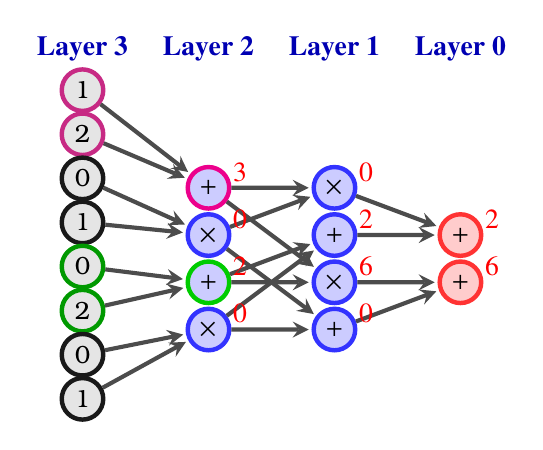
\begin{tikzpicture}[
            % Define styles for different parts of the circuit
            input/.style={circle, ultra thick, draw=gray!20!black, fill=gray!20, minimum size=15pt, inner sep=0pt},
            gate/.style={circle, ultra thick, draw=blue!80, fill=blue!20, minimum size=15pt, inner sep=0pt},
            output/.style={circle, ultra thick, draw=red!80, fill=red!20, minimum size=15pt, inner sep=0pt},
            conn/.style={-stealth, draw=black!70, shorten >=1pt, line width=1.5pt},
            scale=0.8
        ]

        % --- Layer Labels ---
        \node[font=\bfseries, align=center] at (0, 7.45) {\textcolor{blue!70!black}{Layer 3}};
        \node[font=\bfseries, align=center] at (2, 7.45) {\textcolor{blue!70!black}{Layer 2}};
        \node[font=\bfseries, align=center] at (4, 7.45) {\textcolor{blue!70!black}{Layer 1}};
        \node[font=\bfseries, align=center] at (6, 7.45) {\textcolor{blue!70!black}{Layer 0}};

        % --- Layer 0: Input Nodes (8) ---
        % We use a \foreach loop to create the 8 input nodes vertically
        \node[input, draw=magenta!80!black] (l0-1) at (0, 7.5 - 0.7*1) {$\xval{1}$};
        \node[input, draw=magenta!80!black] (l0-2) at (0, 7.5 - 0.7*2) {$\xval{2}$};
        \node[input] (l0-3) at (0, 7.5 - 0.7*3) {$\xval{3}$};
        \node[input] (l0-4) at (0, 7.5 - 0.7*4) {$\xval{4}$};
        \node[input, draw=green!60!black] (l0-5) at (0, 7.5 - 0.7*5) {$\xval{5}$};
        \node[input, draw=green!60!black] (l0-6) at (0, 7.5 - 0.7*6) {$\xval{6}$};
        \node[input] (l0-7) at (0, 7.5 - 0.7*7) {$\xval{7}$};
        \node[input] (l0-8) at (0, 7.5 - 0.7*8) {$\xval{8}$};
        % \foreach \i in {1,...,8} {
        %     \node[input] (l0-\i) at (0, 7.5 - 0.7*\i) {$\xval{\i}$};
        % }

        % --- Layer 1: Gate Nodes (4) ---
        % Alternating between + and x gates
        \node[gate, draw=magenta] (l1-1) at (2, 5.25) {$+$};

        \node[gate] (l1-2) at (2, 4.5) {$\times$};
 
        \node[gate, draw=green!80!black] (l1-3) at (2, 3.75) {$+$};

        \node[gate] (l1-4) at (2, 3.0) {$\times$};

        % --- Layer 2: Gate Nodes (4) ---
        \node[gate] (l2-1) at (4, 5.25) {$\times$};
        \node[gate] (l2-2) at (4, 4.5) {$+$};
        \node[gate] (l2-3) at (4, 3.75) {$\times$};
        \node[gate] (l2-4) at (4, 3.0) {$+$};

        % --- Layer 3: Output Nodes (2) ---
        \node[output] (l3-1) at (6, 4.5) {$+$};
        \node[output] (l3-2) at (6, 3.75) {$+$};


        % --- Connections ---

        % Connections from Layer 0 to Layer 1
        \foreach \i in {1,...,4} {
            \pgfmathtruncatemacro{\j}{2 * \i - 1} % Calculate first source node index
            \pgfmathtruncatemacro{\k}{2 * \i}     % Calculate second source node index
            \draw[conn] (l0-\j) -- (l1-\i);
            \draw[conn] (l0-\k) -- (l1-\i);
        }

        % Connections from Layer 1 to Layer 2
        % This wiring pattern creates a mixing of the signals
        \draw[conn] (l1-1) -- (l2-1);
        \draw[conn] (l1-2) -- (l2-1);

        \draw[conn] (l1-3) -- (l2-2);
        \draw[conn] (l1-4) -- (l2-2);

        \draw[conn] (l1-1) -- (l2-3);
        \draw[conn] (l1-3) -- (l2-3);

        \draw[conn] (l1-2) -- (l2-4);
        \draw[conn] (l1-4) -- (l2-4);

        % Connections from Layer 2 to Layer 3
        \draw[conn] (l2-1) -- (l3-1);
        \draw[conn] (l2-2) -- (l3-1);

        \draw[conn] (l2-3) -- (l3-2);
        \draw[conn] (l2-4) -- (l3-2);

        % Values in gates, layer 2
        \node at (2.5, 5.5) {\textcolor{red}{3}};
        \node at (2.5, 4.75) {\textcolor{red}{0}};
        \node at (2.5, 4.0) {\textcolor{red}{2}};
        \node at (2.5, 3.25) {\textcolor{red}{0}};

        % Values in gates, layer 1
        \node at (4.5, 5.5) {\textcolor{red}{0}};
        \node at (4.5, 4.75) {\textcolor{red}{2}};
        \node at (4.5, 4.0) {\textcolor{red}{6}};
        \node at (4.5, 3.25) {\textcolor{red}{0}};

        % Values in gates, layer 0
        \node at (6.5, 4.75) {\textcolor{red}{2}};
        \node at (6.5, 4.0) {\textcolor{red}{6}};
        \end{tikzpicture}
        \end{center}
        \vspace{-12.5px}
        \begin{gather*}
        \mathsf{add}_2 \; \text{is non-zero}: (\textcolor{magenta}{(0,0)},\textcolor{magenta!80!black}{(0,0,0)},\textcolor{magenta!80!black}{(0,0,1)}), 
        \;
        (\textcolor{green!80!black}{(1,0)},\textcolor{green!60!black}{(1,0,0)},\textcolor{green!60!black}{(1,0,1)}). \\
        \widetilde{\mathsf{add}}_2(\mathbf{X},\mathbf{Y},\mathbf{Z}) = (1-X_1)(1-X_2)(1-Y_1)(1-Y_2)(1-Y_3)(1-Z_1)(1-Z_2)Z_3
        \end{gather*}
    \end{frame}

    \begin{frame}{Reducing to Sum-Check}
        \begin{block}{Remark}
            Note that the operations encodings $\mathsf{add}_i$ and
            $\mathsf{mul}_i$ (and thus MLEs $\widetilde{\mathsf{add}}_i$ and
            $\widetilde{\mathsf{mul}}_i$) do not depend on the solution witness
            $\{\mathbf{x}^{\langle i \rangle}\}_{i \in [d+1]}$, while the gates
            encodings $W_i$ do depend.
        \end{block}

        \textbf{Idea:} Prover sends the claimed value of $\widetilde{W}_0$ (say,
        $D: \{0,1\}^{v_0} \to \mathbb{F}$), then reduce the claim to the next
        around with $\widetilde{W}_1$ (in general, prove the reducing from
        $\widetilde{W}_i$ to $\widetilde{W}_{i+1}$). 
        \begin{figure}
            
\includegraphics[width=0.6\textwidth]{images/lecture_16/where.png}
        \end{figure}
    \end{frame}

    \begin{frame}{Sum-Check Protocol Applied}
        \begin{figure}
            
\includegraphics[width=0.3\textwidth]{images/lecture_16/dicaprio.jpg}
        \end{figure}

        \begin{lemma}
        The following statement holds:
        \begin{align*}
            \widetilde{W}_i(\mathbf{z}) = \sum_{\boldsymbol{b},\boldsymbol{c} \in \{0,1\}^{v_{i+1}}} &\Big[ \widetilde{\mathsf{add}}_i(\mathbf{z},\boldsymbol{a},\boldsymbol{b})(\widetilde{W}_{i+1}(\boldsymbol{b}) + \widetilde{W}_{i+1}(\boldsymbol{c})) \\
            &+ \widetilde{\mathsf{mul}}_i(\mathbf{z},\boldsymbol{b},\boldsymbol{c})\widetilde{W}_{i+1}(\boldsymbol{b})\widetilde{W}_{i+1}(\boldsymbol{c})\Big].
        \end{align*}
        \end{lemma}
    \end{frame}

    \begin{frame}{Why Lemma works?}
        Both sides are multilinear polynomials, thus it suffices to check the equality only over the 
        boolean hypercube $\mathbf{z} \in \{0,1\}^{v_i}$.

        Fix $\mathbf{z}=\mathbf{z}_0 \in \{0,1\}^{v_i}$. Without loss of generality, assume
        $\mathbf{z}_0$ is the addition gate. This way, we reduced the check to:
        \begin{equation*}
            \widetilde{W}_i(\mathbf{z}_0) = \sum_{\boldsymbol{b},\boldsymbol{c} \in \{0,1\}^{v_{i+1}}} \widetilde{\mathsf{add}}_i(\mathbf{z},\boldsymbol{a},\boldsymbol{b})(\widetilde{W}_{i+1}(\boldsymbol{b}) + \widetilde{W}_{i+1}(\boldsymbol{c}))
        \end{equation*}

         According to $\widetilde{\mathsf{add}}$ definition, the only term that is not
        zero in the sum is for
        $(\boldsymbol{b},\boldsymbol{c})=(\mathsf{in}_{1,i}(\mathbf{z}_0),
        \mathsf{in}_{2,i}(\mathbf{z}_0))$. Therefore, our sum is:
        \begin{equation*}
            \widetilde{W}_i(\mathbf{z}_0) = \widetilde{W}_{i+1}(\mathsf{in}_{1,i}(\mathbf{z}_0)) + \widetilde{W}_{i+1}(\mathsf{in}_{2,i}(\mathbf{z}_0))
        \end{equation*}

        \begin{alertblock}{Key Procedure}
            Apply the Sum-Check protocol on the function 
            \begin{equation*}
                \small f_i(\boldsymbol{b}, \boldsymbol{c}; \mathbf{r}_i) = \widetilde{\mathsf{add}}_i(\mathbf{r}_i, \boldsymbol{b}, \boldsymbol{c})(\widetilde{W}_{i+1}(\boldsymbol{b}) + \widetilde{W}_{i+1}(\boldsymbol{c})) + \widetilde{\mathsf{mul}}_i(\mathbf{r}_i, \boldsymbol{b}, \boldsymbol{c})\widetilde{W}_{i+1}(\boldsymbol{b})\widetilde{W}_{i+1}(\boldsymbol{c}).
            \end{equation*}
        \end{alertblock}
    \end{frame}

    \begin{frame}{Caveat with Sum-Check}
        Note that the verifier $\mathcal{V}$ does not know $\widetilde{W}_{i+1}$.

        In fact, he does not need to until the last round, where he needs to
        call an oracle access $\mathcal{O}^{\; f_i}$ at $(\boldsymbol{b}^*,
        \boldsymbol{c}^*) \leftarrowS \mathbb{F}^{2v_{i+1}}$. 
        
        This requires evaluating:
        \begin{itemize}
            \item $\widetilde{\mathsf{add}}_i(\mathbf{r}_i,\boldsymbol{b}^*, \boldsymbol{c}^*)$ --- can be done by $\mathcal{V}$.
            \item $\widetilde{\mathsf{mul}}_i(\mathbf{r}_i,\boldsymbol{b}^*, \boldsymbol{c}^*)$ --- can be done by $\mathcal{V}$.
            \item $\widetilde{W}_{i+1}(\boldsymbol{b}^*)$ and $\widetilde{W}_{i+1}(\boldsymbol{c}^*)$ --- $\mathcal{V}$ needs $\mathcal{P}$'s assistance.
        \end{itemize}

        $\mathcal{P}$ sends two values $z_b =
        \widetilde{W}_{i+1}(\boldsymbol{b}^*)$ and $z_c =
        \widetilde{W}_{i+1}(\boldsymbol{c}^*)$.  If we had only one value to
        check, we could use the standard Sum-Check reduction, but here we have
        two randomnesses!
    \end{frame}

    \begin{frame}{Line Restriction Trick}
        \begin{block}{Proposition}
            Let $\ell: \mathbb{F} \to \mathbb{F}^{v_{i+1}}$ be the line such that
            $\ell(0)=\boldsymbol{b}^*$ and $\ell(1)=\boldsymbol{c}^*$. Then, the prover
            $\mathcal{P}$ sends the univariate polynomial $q(X)$ claimed to be equal to
            $\widetilde{W}_{i+1} \circ \ell$ --- the restriction of
            $\widetilde{W}_{i+1}$ to the line $\ell$. $\mathcal{V}$ checks whether
            indeed $\ell(0)=z_b$ and $\ell(1)=z_c$, then chooses a random point
            $\mathbf{r}^* \xleftarrow{R} \mathbb{F}^{v_{i+1}}$ and checks whether
            $\widetilde{W}_{i+1}(\ell(\mathbf{r}^*)) = q(\mathbf{r}^*)$.
        \end{block}

        This way, the interaction ends with new claim about next(previous) layer
        $\widetilde{W}_{i+1}(\mathbf{r}_{i+1})$ with
        $\mathbf{r}_{i+1}=\ell(\mathbf{r}^*)$.

        In the last round, $\mathcal{V}$ computes
        $\widetilde{W}_d(\mathbf{r}_d)$ on his own.
    \end{frame}

    \begin{frame}{Protocol Summary}
        \begin{itemize}
            \item $\mathcal{P}$ sends function $D: \{0,1\}^{v_0} \to
            \mathbb{F}$, claimed to equal $W_0$.
            \item $\mathcal{V}$ picks random $\mathbf{r}_0 \leftarrowS
            \mathbb{F}^{v_0}$ and lets $m_0 \gets \widetilde{D}(\mathbf{r}_0)$.
            \item For each round $i \in [d]$ do the following:
            \begin{itemize}
                \item Define the $2v_{i+1}$-variate polynomial:
                \vspace{-5px}
                \begin{equation*}
                    \small f_i(\boldsymbol{b}, \boldsymbol{c}; \mathbf{r}_i) = \widetilde{\mathsf{add}}_i(\mathbf{r}_i, \boldsymbol{b}, \boldsymbol{c})(\widetilde{W}_{i+1}(\boldsymbol{b}) + \widetilde{W}_{i+1}(\boldsymbol{c})) + \widetilde{\mathsf{mul}}_i(\mathbf{r}_i, \boldsymbol{b}, \boldsymbol{c})\widetilde{W}_{i+1}(\boldsymbol{b})\widetilde{W}_{i+1}(\boldsymbol{c}).
                \end{equation*}
                \item $\mathcal{P}$ claims $\sum_{\boldsymbol{b},\boldsymbol{c}
                \in \{0,1\}^{v_{i+1}}} f_i(\boldsymbol{b},\boldsymbol{c};
                \mathbf{r}_i) = m_i$.
                \item $\mathcal{P}$ and $\mathcal{V}$ interact using Sum-Check
                protocol until the last round when $\mathcal{V}$ needs to
                evalutate $f_i$ at $\boldsymbol{b}^*, \boldsymbol{c}^*
                \leftarrowS \mathbb{F}^{v_{i+1}}$.
                \item $\mathcal{P}$ and $\mathcal{V}$ compute the line $\ell:
                \mathbb{F} \to \mathbb{F}^{v_{i+1}}$ s.t.
                $\ell(0)=\boldsymbol{b}^*$ and $\ell(1)=\boldsymbol{c}^*$.
                \item $\mathcal{P}$ sends $q$ claimed to equal
                $\widetilde{W}_{i+1} \circ \ell$.
                \item $\mathcal{V}$ validates the last round of sum-check using
                $\ell(0)$ and $\ell(1)$, then chooses $\mathbf{r}^*
                \leftarrowS \mathbb{F}^{v_{i+1}}$ and sets $\mathbf{r}_{i+1}
                \gets \ell(\mathbf{r}^*)$ and $m_{i+1} \gets
                q(\mathbf{r}_{i+1})$.
                \item The check reduces to verifying $\widetilde{W}_{i+1}(\mathbf{r}_{i+1})=m_{i+1}$.
            \end{itemize}
            \item $\mathcal{V}$ directly checks whether
            $m_d=\widetilde{W}_d(\mathbf{r}_d)$.
        \end{itemize}
    \end{frame}

    \begin{frame}[plain, standout]
        \centering
        \LARGE
        \textbf{Thank you for your attention} \\
        
        \vspace{0.2cm} \Huge \ding{170} \large \\
        
        \vspace{1cm}
  
        \href{https://zkdl-camp.github.io/}{\raisebox{-.1em}{\hspace{.025em}\faIcon{globe}}\hspace{.325em}zkdl-camp.github.io} \\
  
        \href{https://github.com/ZKDL-Camp}{\raisebox{-.1em}{\hspace{.025em}\faIcon{github}}\hspace{.325em}github.com/ZKDL-Camp}
        
        \begin{center}
            
\includegraphics[width=0.15\textwidth]{images/logo.png}
        \end{center}
    \end{frame}
\end{document}
